\appendix
\chapter{m-maps}
\label{mmapsappendix}
\newlength{\mwidths}
\setlength{\mwidths}{0.3\linewidth}

Looking at the m-maps we can say that, 
$m_5$ and $m_8$ are very noisy. m1,m2,m4 have similar information and
$m_6,m_7,m_9$ have similar information. And $m_9$ is also more noisier than $m_7$.
Therefore, We choose $m_1$, $m_3$ and $m_7$.

\begin{figure}[htbp]
  \centering
 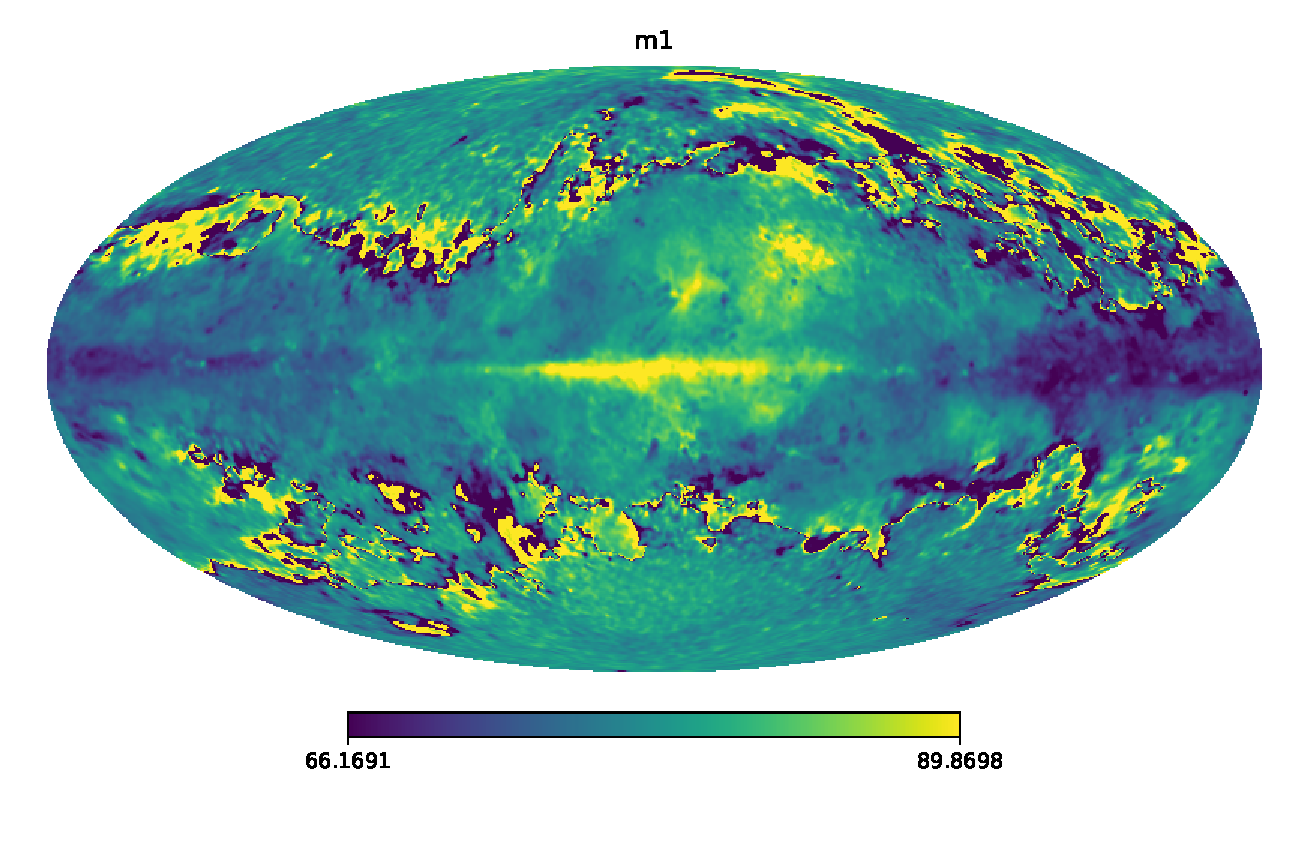
\includegraphics[width=\mwidths]{m-maps/map_m1.eps}
 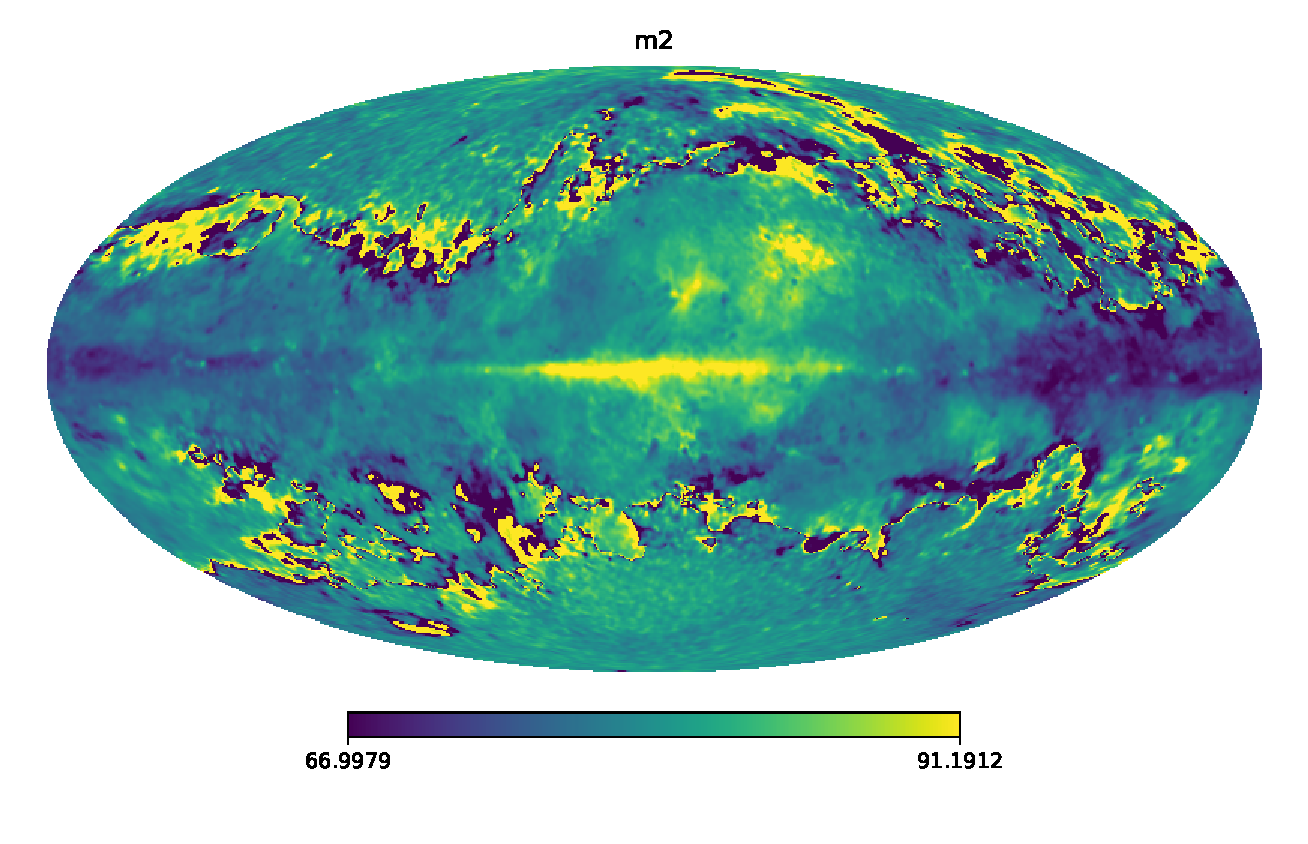
\includegraphics[width=\mwidths]{m-maps/map_m2.eps}
 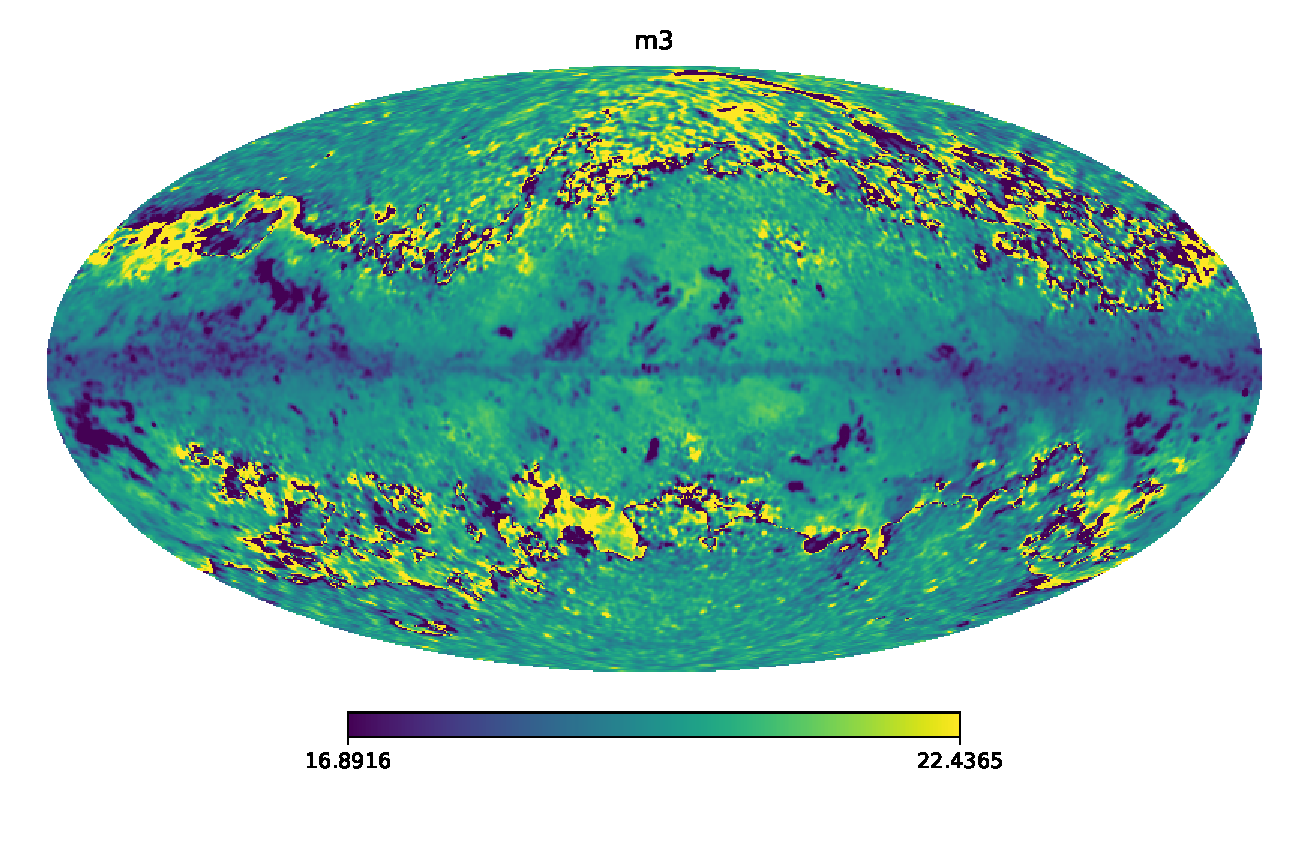
\includegraphics[width=\mwidths]{m-maps/map_m3.eps}
 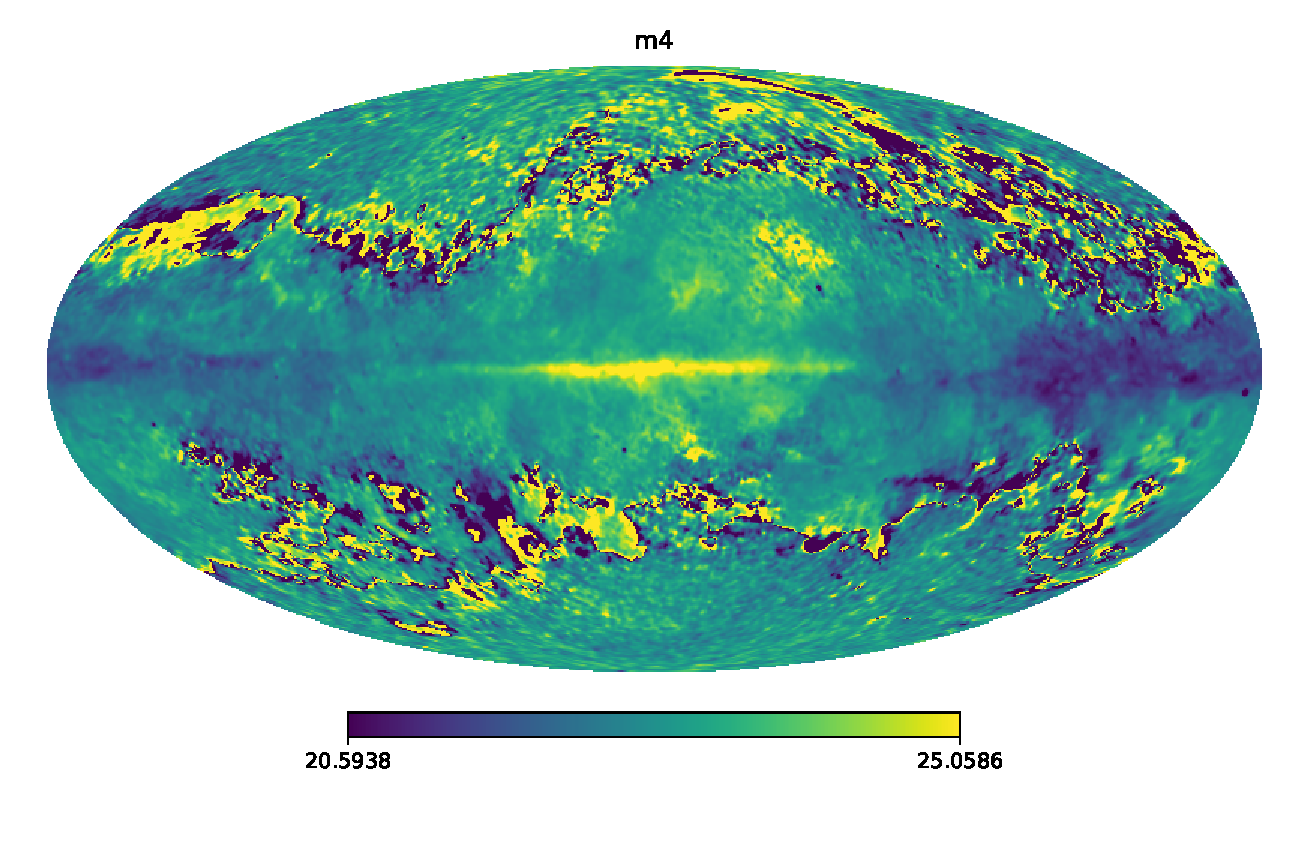
\includegraphics[width=\mwidths]{m-maps/map_m4.eps}
 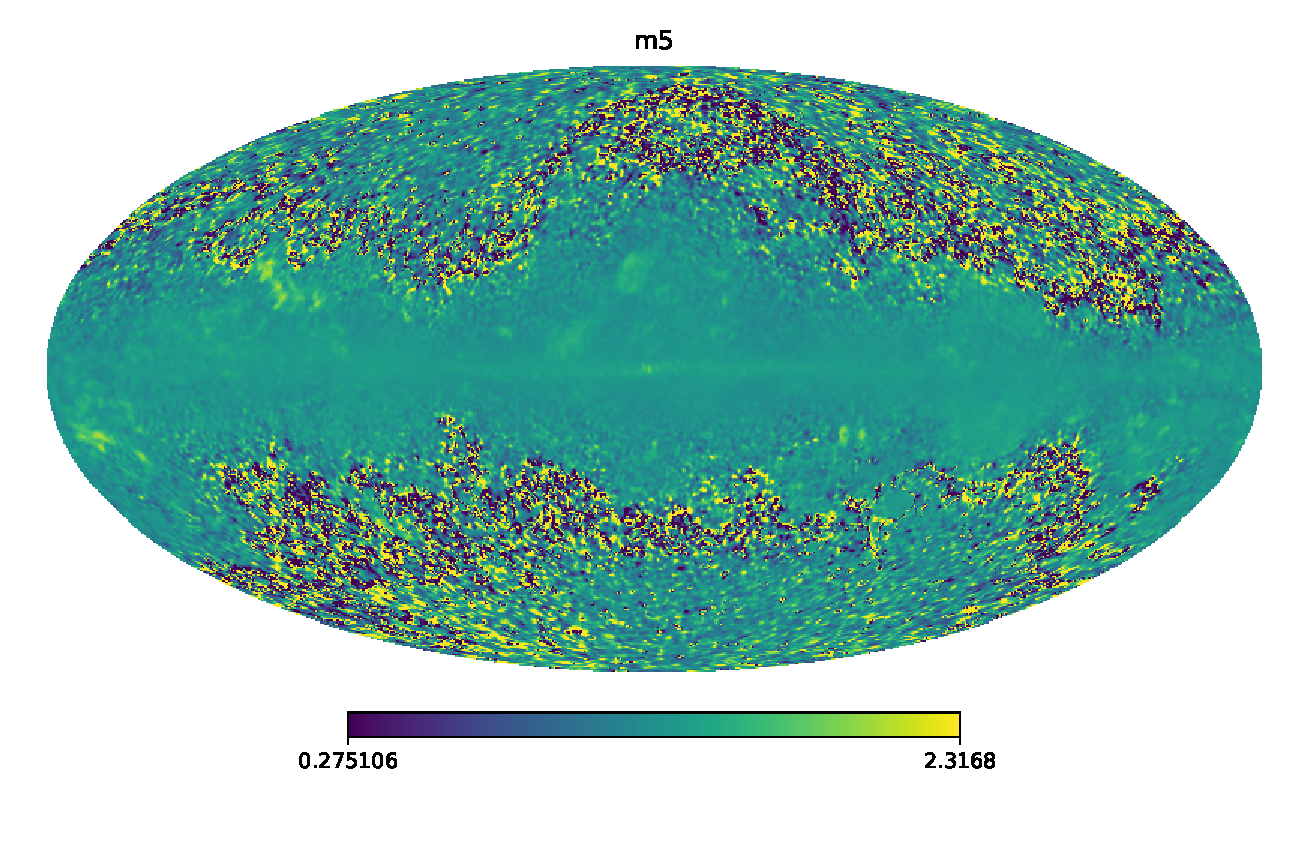
\includegraphics[width=\mwidths]{m-maps/map_m5.eps}
 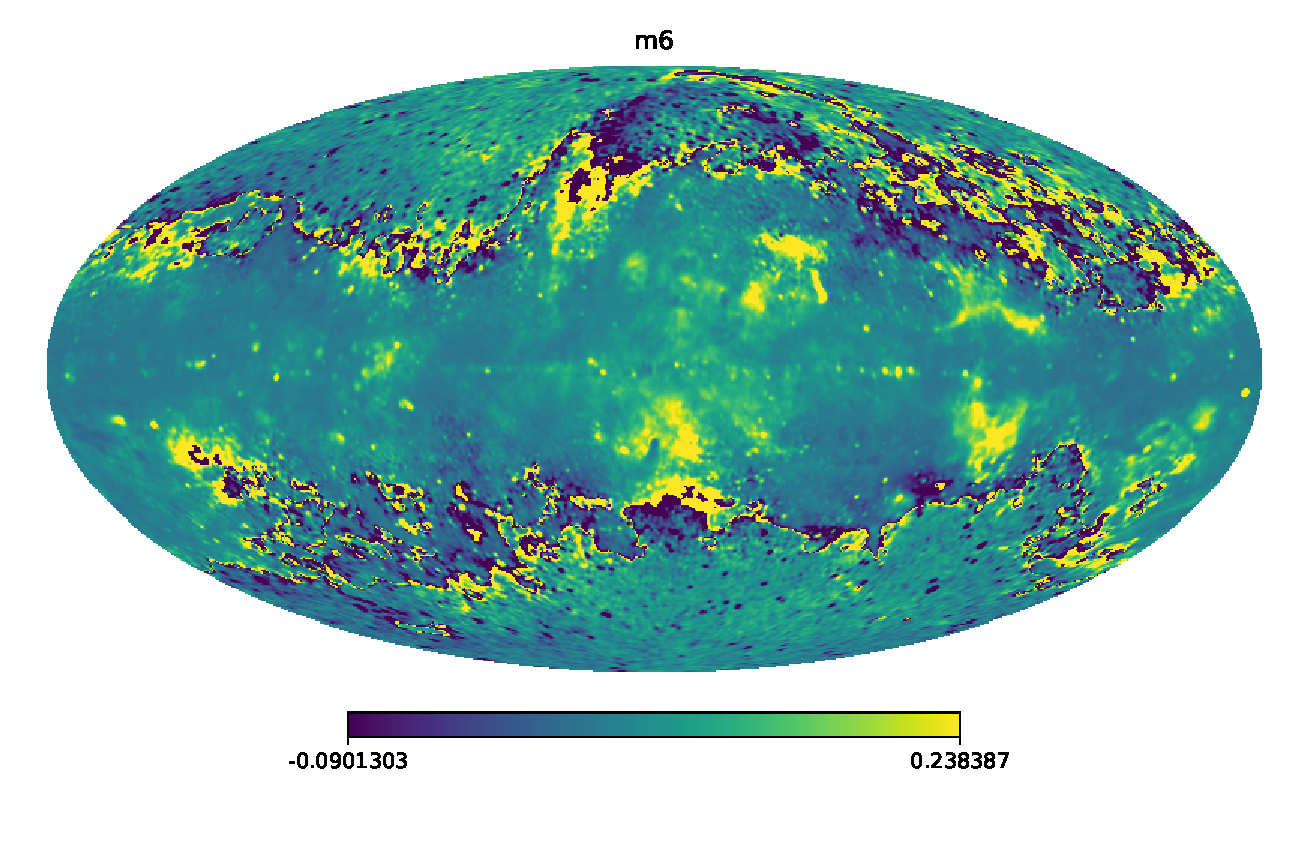
\includegraphics[width=\mwidths]{m-maps/map_m6.eps}
 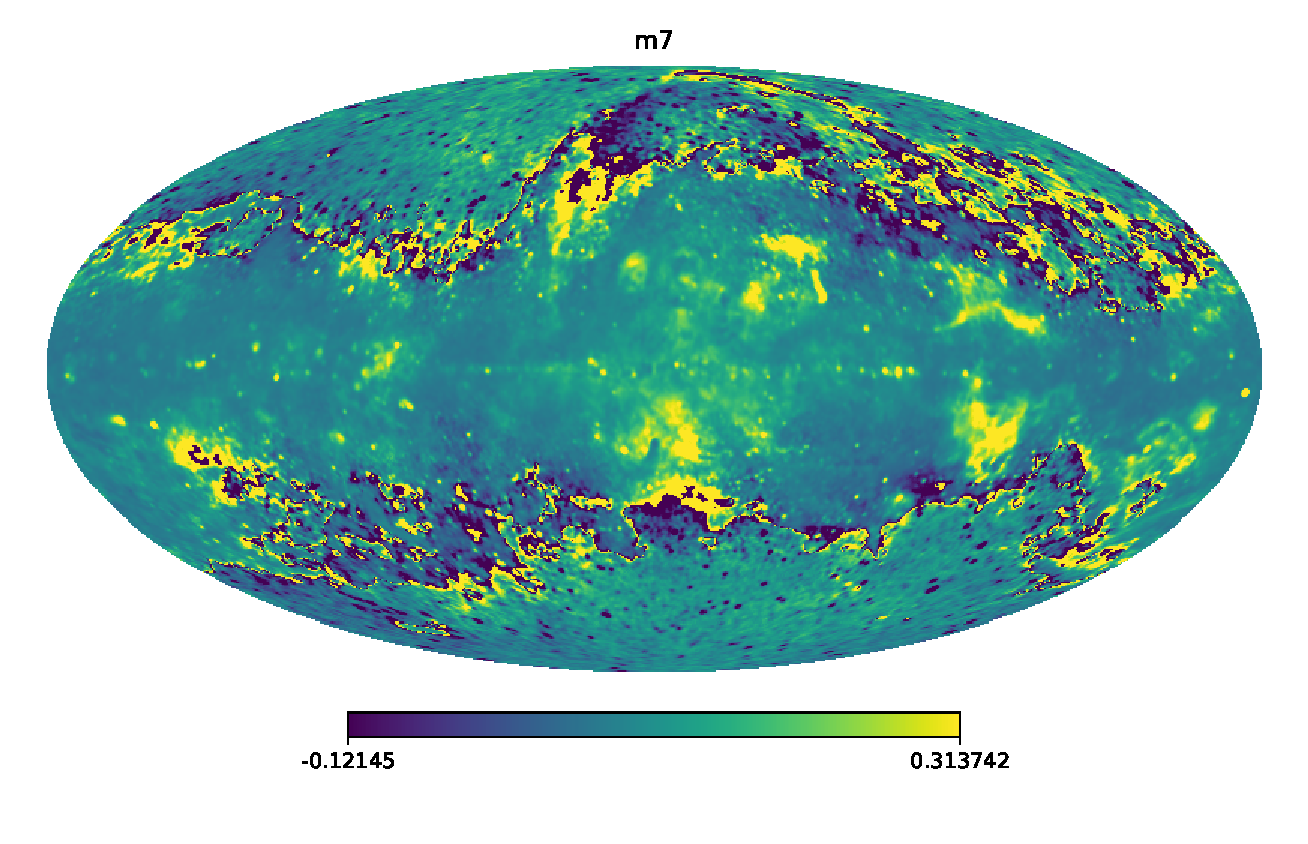
\includegraphics[width=\mwidths]{m-maps/map_m7.eps}
 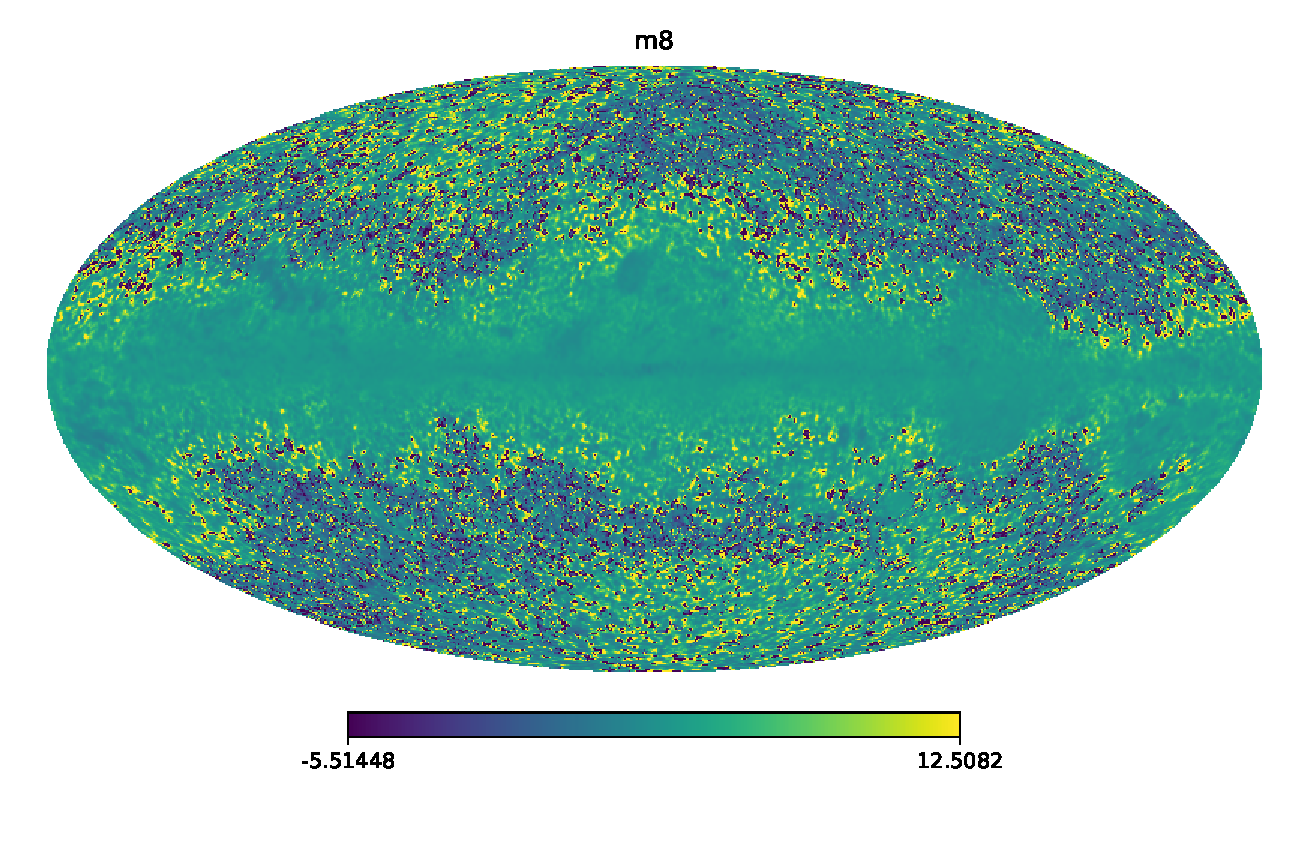
\includegraphics[width=\mwidths]{m-maps/map_m8.eps}
 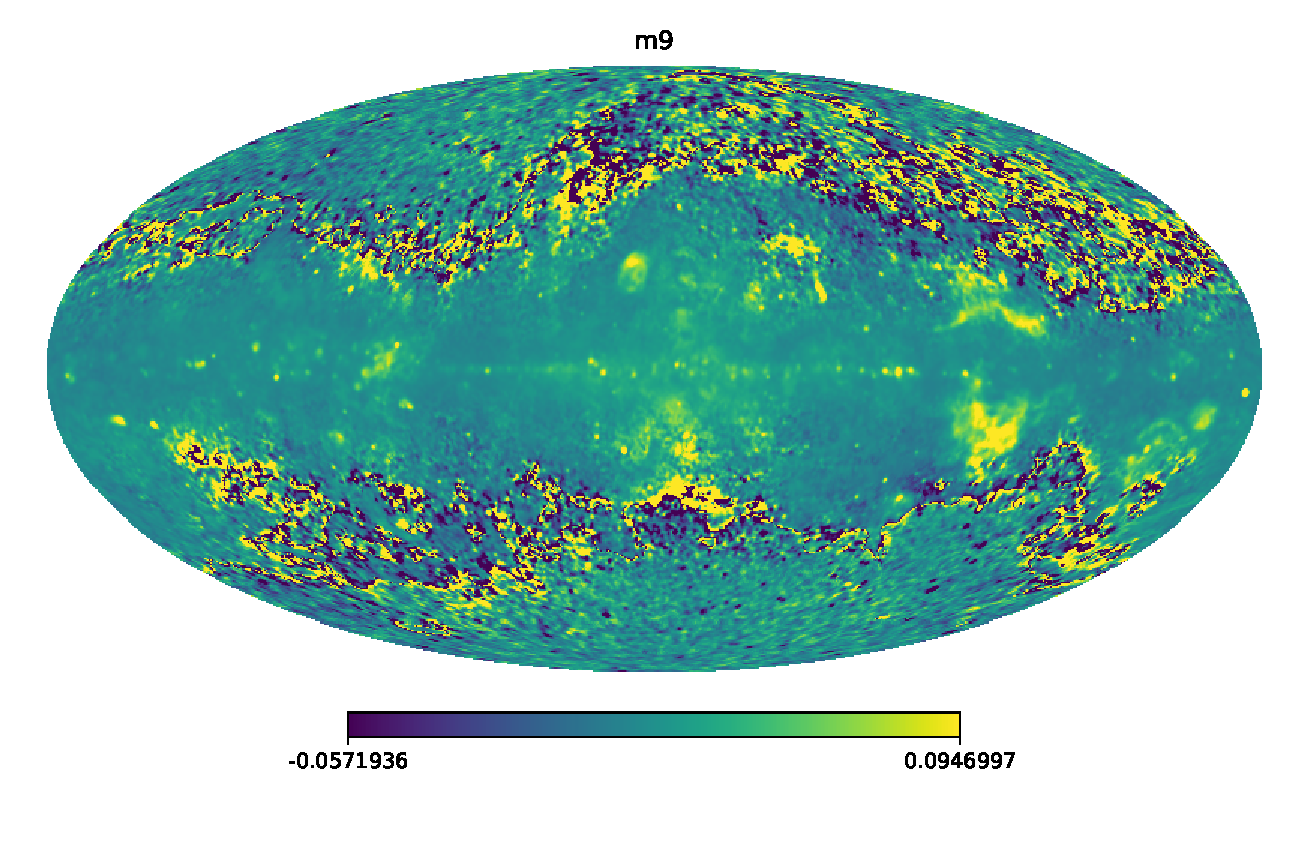
\includegraphics[width=\mwidths]{m-maps/map_m9.eps}
 \caption{The m-maps for planck data (these maps are plotted only from 5 to 95
   percentile to avoid the outliers from scaling the plot)}
\end{figure}
%%% Local Variables:
%%% mode: latex
%%% TeX-master: "thesis"
%%% End:
